\hypertarget{__rb__rotate_8c}{
\section{\_\-rb\_\-rotate.c File Reference}
\label{__rb__rotate_8c}\index{_rb_rotate.c@{\_\-rb\_\-rotate.c}}
}


\subsection{Detailed Description}
\begin{Desc}
\item[For internal use only.]
This file contains the implementation of the \hyperlink{group__dbprim__rbtree_ga15}{\_\-rb\_\-rotate()} function, used to perform a tree node rotation for tree balancing.\end{Desc}


Definition in file \hyperlink{__rb__rotate_8c-source}{\_\-rb\_\-rotate.c}.

{\tt \#include \char`\"{}dbprim.h\char`\"{}}\par
{\tt \#include \char`\"{}dbprim\_\-int.h\char`\"{}}\par


Include dependency graph for \_\-rb\_\-rotate.c:\begin{figure}[H]
\begin{center}
\leavevmode
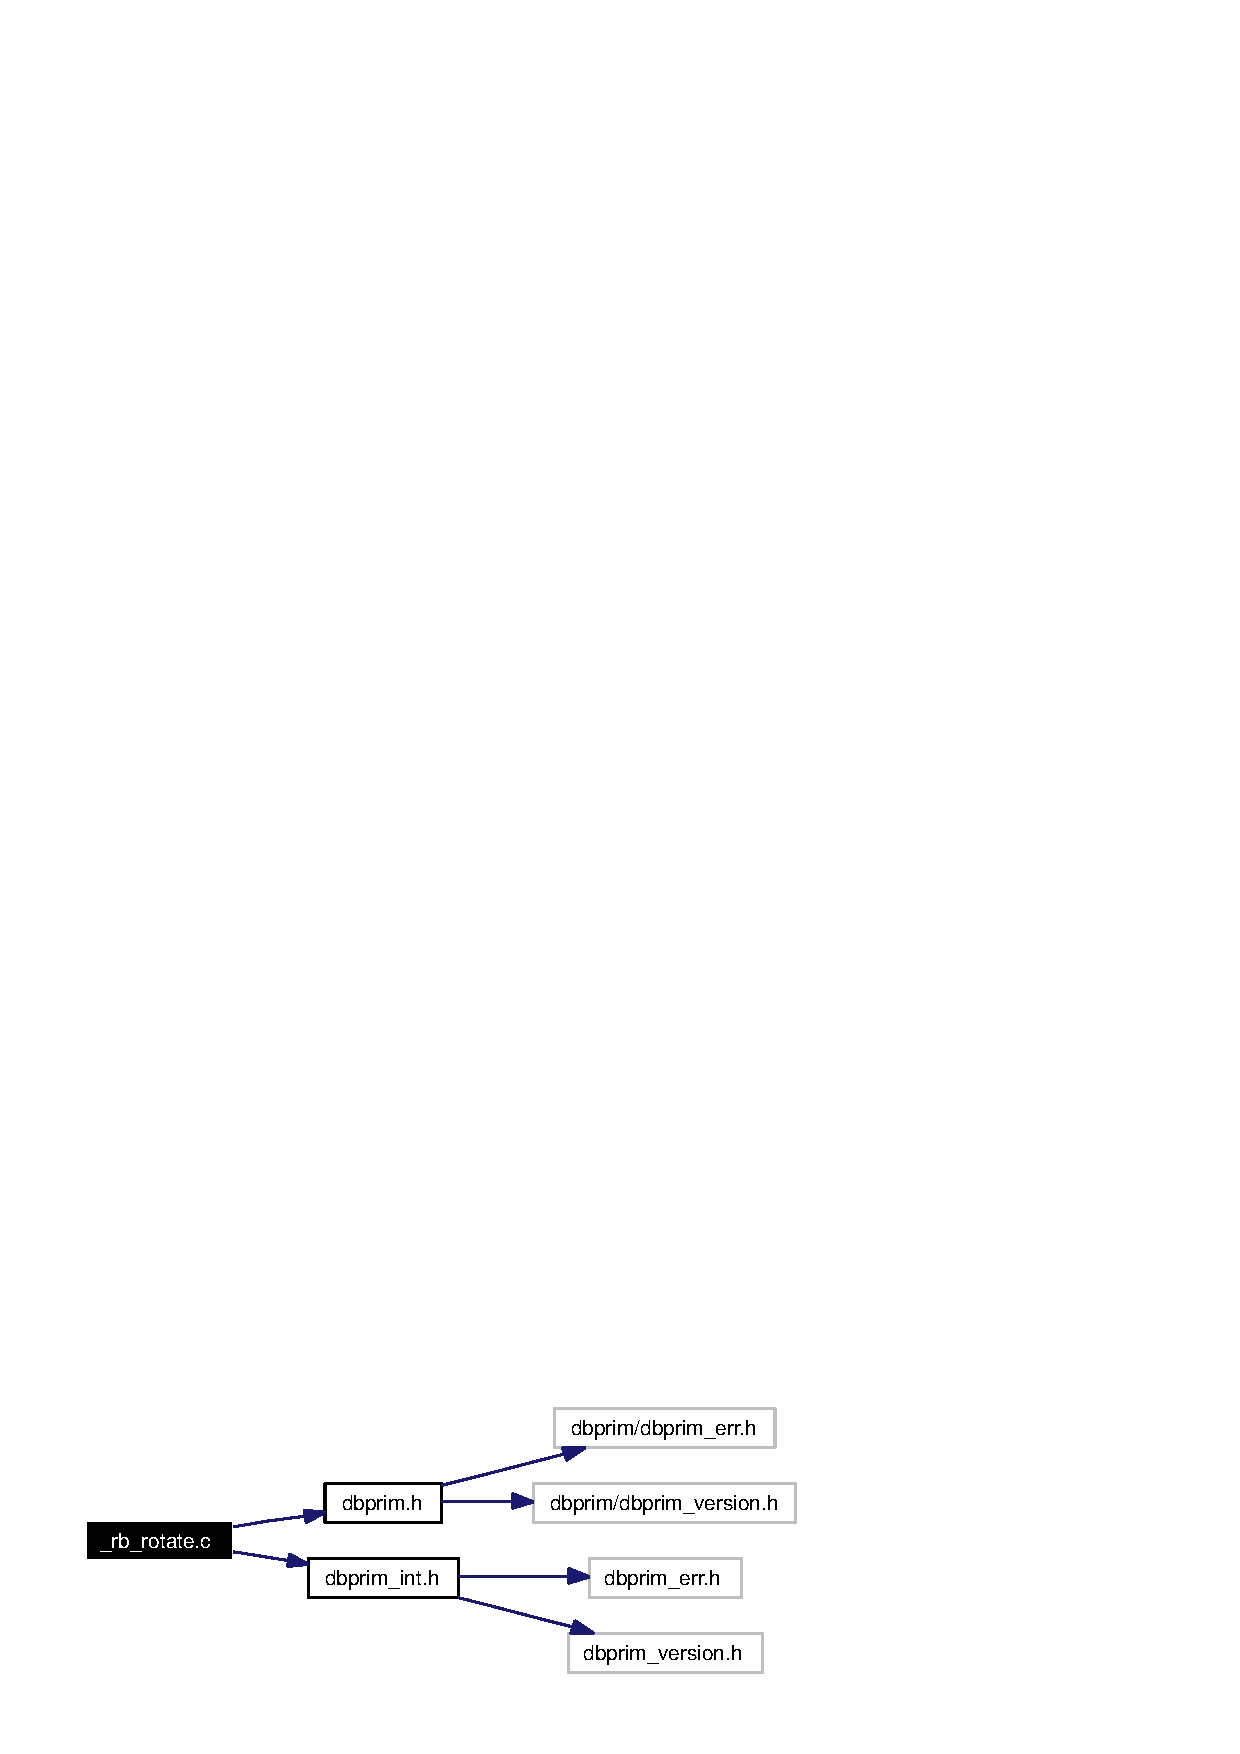
\includegraphics[width=193pt]{__rb__rotate_8c__incl}
\end{center}
\end{figure}
\subsection*{Functions}
\begin{CompactItemize}
\item 
void \hyperlink{group__dbprim__rbtree_ga15}{\_\-rb\_\-rotate} (\hyperlink{struct__rb__tree__s}{rb\_\-tree\_\-t} $\ast$tree, \hyperlink{struct__rb__node__s}{rb\_\-node\_\-t} $\ast$child)
\begin{CompactList}\small\item\em Rotate tree nodes. \item\end{CompactList}\end{CompactItemize}
